\documentclass[border=3pt,tikz]{standalone}
\usepackage{amsmath}
\usetikzlibrary{arrows.meta}
\usetikzlibrary{calc}
\usetikzlibrary{math}
\usepackage{mathtools}
\begin{document}
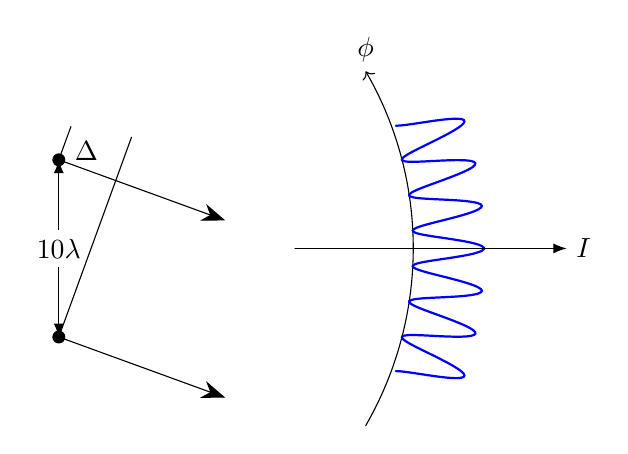
\begin{tikzpicture}[line cap=round, scale=1.5]
    % 관찰자가 움직일때의 도플러 효과
    \def\l{0.15}
    \def\th{20}
    \def\R{3}
    \def\ph{20}
    %\def\k{30 *180/3.141592}
    \def\k{200}
    \coordinate (P1) at (0, {\l*5});
    \coordinate (P2) at (0, {-\l*5});
    \coordinate (A0) at ({-\ph-10}:\R); 

    \filldraw[] (P1) circle (0.05) ;
    \filldraw[] (P2) circle (0.05) ;
    \draw[Latex-Latex] (P1) -- node[ midway,fill=white] {$10\lambda$} (P2);
    \node[xshift=10, yshift=3] at (P1) {$\Delta$};
    \draw [] (P2) -- ++ ({90-\th}:{\l*12});
    \draw [] (P1) -- ++  ({90-\th}:{\l*2});
    \draw [-{Stealth[length=3mm]}] (P1) -- ++ (-\th: {\l*10});
    \draw [-{Stealth[length=3mm]}] (P2) -- ++ (-\th: {\l*10});
    \draw [->](A0) arc ({-\ph-10}:{\ph+10}:\R) node [above ]{$\phi$}; 
    \draw[domain={-\ph}:\ph,variable=\t,samples=200,smooth, thick,blue] 
        %\def\Q{{sin(2*\t) + \R}};
        % plot (\t:{ \R+0.6*(cos(\k*(sqrt((\R*cos(\t))^2 + (\R*sin(\t)+5*\l)^2))-\k*(sqrt((\R*cos(\t))^2 + (\R*sin(\t)-5*\l)^2))))^2});
        plot (\t:{ \R+0.6 * (cos(1200*10*\l*sin(\t)))^2});
    
    \draw[-Latex] ({\R-1}, 0) -- ({\R+1.3}, 0) node [right] {$I$};
    \end{tikzpicture}
\end{document}
